\documentclass[bachelor]{thesis-uestc}

\title{基于语法树的文档级关系预测算法设计与验证}{Design and Verification of Document-level Relation Extraction Algorithm Based on Syntax Tree}
\author{朱旭东}{Xudong Zhu}
\advisor{康昭\chinesespace 副教授}{Dr. Zhao Kang}
\school{计算机科学与工程学院(网络空间安全学院)}{School of Computer Science and Engineering}
\major{计算机科学与技术}{Computer Science and Technology}
\studentnumber{2020080902004}

\usepackage{graphicx}

\begin{document}

\makecover

\begin{chineseabstract}
    文档级关系抽取旨在识别单个文档中实体对之间的关系。
    它需要处理多个句子并对这些句子进行推理。
    最先进的文档级关系抽取使用图形结构来连接文档中的实体,来捕获文档中的实体对的交互。 
    但是这些方法没有充分利用在句子级关系抽取中被充分研究的语法信息。
    在本文中我们以将语法树融合到文档级关系抽取中为主要研究内容,重点研究了使用依赖语法树,依存语法树进行文档级关系抽取算法的实现,以及怎么调整依赖语法树和依存语法树的在文档级关系抽取中的权重问题。
    我们利用依存语法树来聚合整个句子信息,并为目标实体对选择有指导意义的句子。
    同时我们利用依赖语法树对整个文档进行细粒度的分析,并选择其中重要的单词增强目标实体对的信息。
    文档级关系抽取将同时利用依赖语法树和依存语法树进行预测。
    通过在不同领域的数据集上的实验结果证明了该方法的有效性。 


\chinesekeyword{文档级关系抽取,依赖语法树,依存语法树,语法树融合}
\end{chineseabstract}

\begin{englishabstract}
    Document-level Relation Extraction (DocRE) aims to identify relation labels between entity pairs within a single document. 
    It requires handling several sentences and reasoning over them.
    State-of-the-art DocRE methods use a graph structure to connect entities across the document to capture interaction between entity pairs in the document.
    However, this is insufficient to fully exploit the rich syntax information in the document, which is widely used in sentence-level Relation Extraction(RE). 
    In this thesis, we focus on integrating syntax trees into DocRE as the main research topic, and investigate the effective and effient implementation of DocRE algorithms using dependency syntax tree and constituency syntax tree, as well as how to adjust the weight of dependency syntax tree and constituency syntax tree in the extraction. 
    It uses constituency syntax to aggregate the whole sentence information and select the instructive sentences for the pairs of targets. 
    Meanwhile, it exploits the dependency syntax in a graph structure with constituency syntax enhancement and selects the most important words between entity pairs based on the dependency graph to enhance the information of target entity pairs. 
    Finally, DocRE will integrate the dependency syntax and constituency syntax to predict.
    The experimental results on datasets from various domains demonstrate the effectiveness of the proposed method.


    \englishkeyword{Document-level Relation Extraction, Constituency Syntax, Dependency Syntax, Syntax Tree Fusion}
\end{englishabstract}

\thesistableofcontents

\chapter{绪\hspace{6pt}论}
\section{研究的背景}
关系提取是信息提取中的一项关键任务,旨在对非结构化文本中实体对之间的关系模式进行建模。
有两种特定的场景:句子级关系提取和文档级关系提取。
与句子级关系提取 \cite{sentenceRE-Dixit, sentenceRE-Lyu} 不同,文档级关系提取识别文档中实体对之间的关系标签。
因此,文档级关系提取更好地满足了实际需求,最近受到了越来越多的关注。\par

文档级关系提取面临的一个巨大障碍是推断长句中实体对的关系,这是因为长句中通常包含不相关甚至有噪声的信息。
图 \ref{fig_exam}是一个例子,它包括一对来自同一文档中的句子级关系和文档级关系。
为了推断Louis Chollet和Conservatoire de Paris之间的关系,模型应该能够排除不相关实体的影响,并找出句子2中的“He”一词指的是“Louis Cholet”。
然而,由于现有的文档级关系提取模型 \cite{bai-etal-2021-syntax} 经常会被大量不相关的信息所淹没,从而无法捕捉到类似的关键信息。 \par

最近,预训练语言模型在许多下游任务中显示出巨大的潜力。
一些工作\cite{ye-etal-2020-co-ferential, zhou2021document}试图通过预训练语言模型隐含地捕捉到实体之间的这种交互,但是最近的研究 \cite{sundaraman2019syntax, bai-etal-2021-syntax, liu2023document} 表明通过预训练语言模型隐式学习的交互与黄金标记之间仍然存在很大差距。
因此,对于文档级关系提取,隐含地学习一个有指导意义的上下文是不够的。
而语法信息在句子级关系提取 \cite{xu-etal-2016-improved, qin-etal-2021-relation} 中得到了广泛的应用,但在文档级关系提取的场景下尚未得到充分的探索。
因此本文通过融合语法信息作为辅助,来改进文档级关系提取。\par

\begin{figure}
    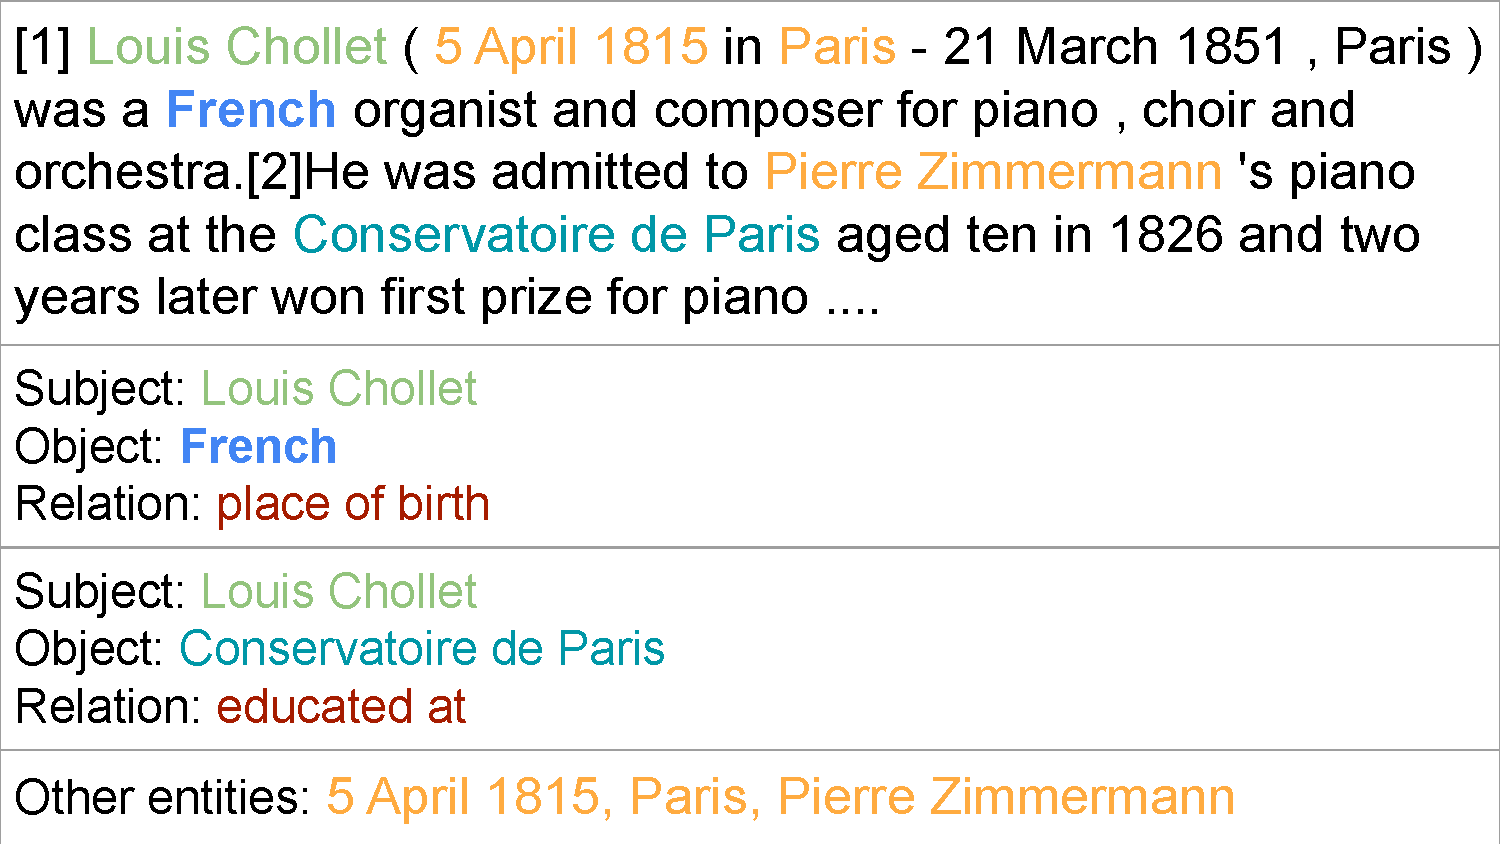
\includegraphics[height=0.5\textwidth]{misc/example1.pdf}
    \label{fig_exam}
    \caption{
        来自DocRED数据集的一对句子级关系实例和文档级关系实例。
        我们将不同的实体和关系标注为不同的颜色来突出不相关实体对关系预测的影响。
    }
\end{figure}

\section{研究的主要内容}

\section{研究的主要贡献与创新}

\section{研究的结构安排}

\chapter{关系抽取研究}
\newpage
1

\newpage

\chapter{语法信息研究}
\newpage
1
\newpage
\chapter{基于语法树的文档级关系抽取研究}
\newpage
1
\newpage
\chapter{基于语法树的文档级关系抽取实验结果}
\newpage
1
\newpage
\chapter{结论}
\thesisacknowledgement
在攻读计算机学士学位期间,首先热烈感谢我的导师康昭教授。经过风风雨雨的研究,我得到了他的无私关怀和支持。在此特别表达感谢之情。我还要感谢我的一直以来的帮助者们,包括学院的老师、同学、同事,以及所有支持和关心我的人。我也要感谢我的家人,他们给予我强大的内心支持和生活的安定和稳定。

\thesisappendix


% Uncomment to list all the entries of the database.

\thesisbibliography{reference}

%
% Uncomment following codes to load bibliography database with native
%\bibliography command.

%\bibliographystyle{thesis-uestc}
%\bibliography{reference}


%\thesistranslationoriginal
%\section{The OFDM Model of Multiple Carrier Waves}

%\thesistranslationchinese
%\section{基于多载波索引键控的正交频分多路复用系统模型}

\end{document}
